% \documentclass[./Mate2.tex]{subfiles}
%\usepackage[letterpaper]{geometry}% Custom margins
%\usepackage{graphicx}
%\graphicspath{{\subfix{../Images/}}}
%\setlength{\parindent}{0pt}
% \title{Portada}
% \author{Julio C. Melchor P.\thanks{{\tt julio.melchor@rafaeldiazserdan.net}}}
% \date{v1.0, \today}
%\usepackage[dvipsnames]{xcolor} % Required for custom color
\usepackage{color,colortbl}
\usepackage[utf8]{inputenc}
\usepackage{geometry} % Custom margins
\usepackage[spanish]{babel}
\usepackage{adjustbox,dashbox}
\usepackage{array}
\usepackage{tikz,pgfplots,pgfkeys}
\usepackage{forest,mathtools,siunitx}
\usepackage{amsfonts, amssymb, amsxtra, amsmath, amsbsy}
\usepackage{newclude}
\usepackage{ifthen}
\usepackage{float}
\usepackage{fancybox}
\usepackage{graphicx,tabularx}
\usepackage{multicol,multirow}
\usepackage{enumitem} % Customising the numbered lists
\usepackage{xhfill} % Making the pink block not extend beyond the margin
\usepackage{nameref} % reference the names of the sections
\usepackage{caption,capt-of}
\usepackage[normalem]{ulem} % Dashed lines in appendix
\usepackage{ragged2e} % Ragged left
\usepackage{booktabs}
\usepackage[unboxed]{cwpuzzle}
\usepackage[colorlinks = true,linkcolor = blue]{hyperref}
\usepackage{subfiles}
\usepackage{wrapfig}
\input{insbox}
\usepackage{etoolbox}
\usepackage{mwe}
\usepackage{comfortaa}
\usepackage[T1]{fontenc}
\renewcommand*\oldstylenums[1]{{\firaoldstyle #1}}
\usepackage[T1]{fontenc}
\usepackage{pythontex}
\usepackage{polynom}
\usepackage{longdivision}

 % Imports all the required packages. See Functional/%Packages.tex for more detailS
%\newgeometry{left=0mm,top=50mm,bottom=0mm,right=0mm}
% \begin{document}
\thispagestyle{empty}
\begin{center}
    \vspace{4cm}
    {\Huge Matem\'aticas 2}\\
    \vspace{1cm}
    \normalsize
    \textbf{\large Cuaderno de trabajo}\\
    para los alumnos de 2$^\circ$ de  Secundaria\\
    en el curso durante el ciclo escolar\\
    \textbf{2022-2023}\\
    \vspace{2cm}
    \small POR\\
    \Large J. C. Melchor Pinto\\[0.5em]
    \normalsize Profesor de asignatura en\\
    \vspace{2cm}
    
\includegraphics[width=4cm]{../Images/LOGO_RDS_nobg}\\
    \vspace{1cm}
\end{center}
%\vspace{1cm}
%\include*{Functional/TitlePage}
%\hspace{-16mm}
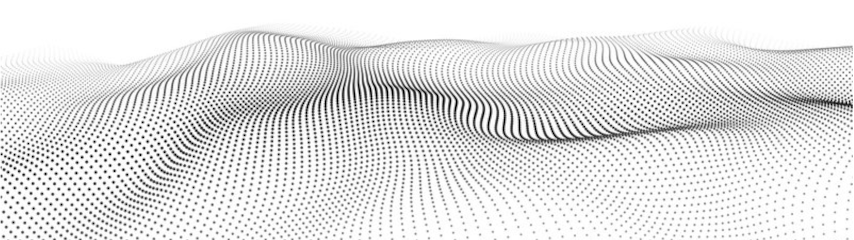
\includegraphics[width=1.1\textwidth]{../Images/cover_bg}
%\restoregeometry
% \end{document}